\chapter{Software Architecture Overview}
\label{overview}

The system developed in the course of our work can be divided into three main components:

\begin{enumerate}
\item A \emph{Client Web Interface}, where all the provided services implemented in our system can be seen and requested by any user. This interface is also responsible for handling the clients' requests, namely invoking the desired services from different implementations of the \emph{Web Service}, calling the \emph{Voter} and presenting the final result to the user.

\item One version of the proposed \emph{Web Service}, responsible for computing the number of insulin units a given patient must take, according to the parameters specified in the client's interface.

\item The \emph{Voter} system, responsible for selecting the adequate number of insulin units a patient must take, given the answers provided by each of the \emph{Web Services} requested by the client's interface.
\end{enumerate}

In figure \ref{architecture} we present the architecture described and implemented in our system. Even though the \emph{Voter} and the \emph{Web Service} are running in the same machine, in this figure we decided to represent seperatly to show their interaction.

\begin{figure}[H]
    \centering
	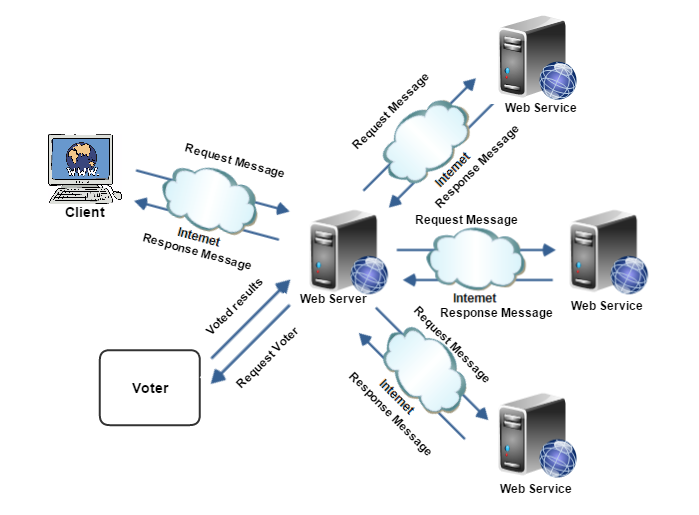
\includegraphics[keepaspectratio=true, scale=0.5]{Overview.png}
	\caption{Software Architecture of our Application}
	\label{architecture}
\end{figure}

To use the developed system, the user must make use of the \emph{Client Interface} provided, select the operation that he/she wants to invoke, input the necessary and requested parameters and  press the button \emph{"Calculate Insuline Dose"} to request the number of insulin units adequate for the parameters specified.

When the user presses this button a request is triggered to our \emph{Web Server} (hosting the \emph{Web Interface}). The \emph{Web Server} then randomly selects three \emph{Web Services}\footnote{From a previously generated list of \emph{Web Services}} and makes the desired request.

Then, for of the selected \emph{Web Services} the \emph{Server} either gets a response in feasible time or identifies the occurrence of a \emph{timeout} in the \emph{Web Service side}.

After receiving all the responses from the \emph{Web Services}, the \emph{Server} invokes the \emph{Voter}. The \emph{Voter System} collects all the responses from the \emph{Web Services} and selects the majority response which is presented to the user. In case a majority consensus can not be achieved the entire process is repeated, i.e., the request is sent to three different \emph{Web Services}  until there is no feasible time to retrieve the answer to the user. At that point a message is displayed in the \emph{Web Interface} reporting the situation (impossibility of obtaining a valid consensual final value).